\chapter{Methode}
In dit hoofdstuk worden de bouwblokken van de fietssimulatie aangehaald. Daarna bekijken we de verschillende stappen, zoals preprocessing, ..., die aanwezig zijn in de cadanscontroller. Vervolgens wordt er een stochastisch keuzemodel voorgesteld dat de willekeurigheid van een mens moet simuleren. Ten slotte worden verschillende methodes besproken die ervoor zorgen dat een model zich snel kan aanpassen.
\section{De fietssimulatie}
Er wordt een simulatie gemaakt die de toestand van de fiets zo goed mogelijk benadert. Er zal geen rekening gehouden worden met het manoeuvreren van de fiets of met tegenwind. Enkel de relevante meetwaarden worden bijgehouden. De simulatie is geparametriseerd om eenvoudig verschillende scenario’s te testen. De simulatie is gebaseerd op werk van \cite{hardware implementation}.
\\\\
Het voordeel van de fietssimulatie is de enorme flexibiliteit. Uren aan data kunnen in een mum van tijd gegenereerd worden, waardoor het makkelijk is om verschillende testen uit te voeren. Hiervoor moeten slechts enkele instellingen aangepast worden. Het is ook mogelijk om slechts een enkele parameter aan te passen tijdens testen, terwijl de rest constant blijft (\textit{ceteris paribus}), wat praktisch onmogelijk is in een veldtest. Omdat de simulatie bovendien een duidelijke referentie genereert voor de FCC (output van het fietsersmodel), kan de performantie van de cadanscontroller op een kwantitatieve manier worden geëvalueerd. Tijdens een veldtest zou de fietser alleen kwalitatief kunnen aangeven of hij of zij de voorspelde cadans goed vindt. 
\subsection*{Modelleren van het fietserkoppel}
Het fietserkoppel wordt gemodelleerd als een sinusfunctie met twee pieken per omwenteling van de trapas (2 benen), met het DC-koppel van de fietser als parameter. \gls{dc} binnen de signaaltheorie wordt gezien als het signaal op nul Hertz. Het DC-koppel is vergelijkbaar met het gemiddeld koppel.
\\
\begin{gather*}
 T_{cy} = \gls{t_dc}(1+sin(2\theta_{cr}-\frac{\pi}{6}))
\end{gather*}
\\
Uit deze formule is het ook meteen duidelijk dat het DC-koppel ook het vermogen-equivalent koppel is. Dat wil zeggen dat het DC-koppel gedurende een volledige omwenteling van de trapas evenveel arbeid levert als het fietserkoppel.
\\
\begin{align*}
\int_{0}^{2\pi} T_{cy}(1+sin(2x-\frac{\pi}{6})) dx &= T_{cy} \int_{0}^{2\pi}(1+sin(2x-\frac{\pi}{6})) dx\\
&= T_{cy} \left[x-\frac{1}{2}sin(\frac{1}{3}(6x+\pi))\right]_0^{2\pi}\\
&= 2\pi \ T_{cy}
\end{align*}
\\
\noindent
Het gemiddelde koppel geleverd door de fietser wordt gemodelleerd als een proportionele regelaar. Het doel is om een bepaalde snelheid, $v_{ref}$, te behalen. Hoe groter het verschil is tussen de referentiesnelheid en de eigenlijke snelheid, hoe meer kracht er geleverd zal worden. Als deze referentiesnelheid overschreden wordt, dan zal er geen koppel meer geleverd worden. Dit wordt ook wel \textit{freewheelen} genoemd. Om de kracht van de actor te limiteren, wordt er een maximum koppel ingesteld ($T_{dc,max}$) naar gelang de huidige cadans (\gls{omega_cr}). Zo wordt er meer kracht geleverd wanneer de cadans laag is, net zoals in de werkelijkheid. \gls{k} bepaalt de agressiviteit van de regelaar. De formules zien er als volgt uit:

\begin{gather*}
\gls{t_dc_max} = \frac{-\omega_{cr}}{2}+60 \tab (Figuur\ \ref{fig:koppeltoerentalkarakteristiek}) \\
T_{dc} = min(T_{dc,max},max(0,-K*(v_{bike}-v_{ref}))
\end{gather*}
\\
\begin{figure}
  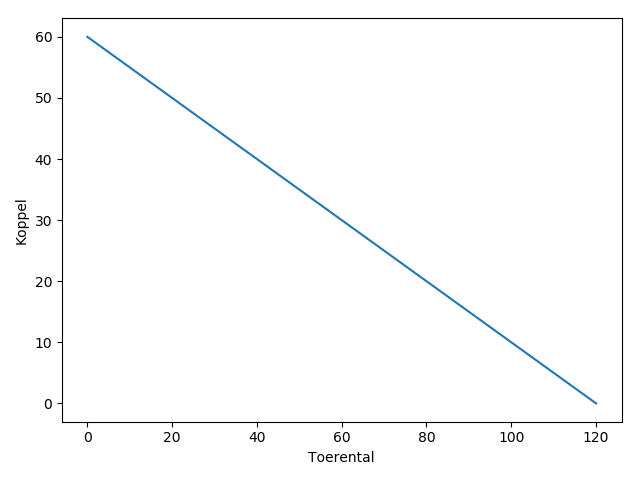
\includegraphics[width=\linewidth]{images/koppel-toerentalkarakteristiek.png}
  \caption{De koppel-toerentalkarakteristiek}
  \label{fig:koppeltoerentalkarakteristiek}
\end{figure}
\\
\noindent Figuren \ref{fig:menselijkkoppelverloop} en \ref{fig:gesimuleerdkoppelverloop} tonen een menselijk koppelverloop en gesimuleerd koppelverloop, gesampled aan 10 Hz. Zoals te zien is het gesimuleerde koppel heel consistent. Het menselijk koppel volgt duidelijk een cyclische functie, maar vertoont vormen van inconsistentie. Merk wel op dat er telkens een afwisseling is van een hoge en een lage piek. Dit wijst op een dominant been. Figuur \ref{fig:gesimuleerde koppel dominant been} toont een gesimuleerd koppelverloop van een fietser met een dominant been.
\\\\
\begin{figure}[t!]
\centering
\begin{subfigure}{.5\textwidth}
  \centering
  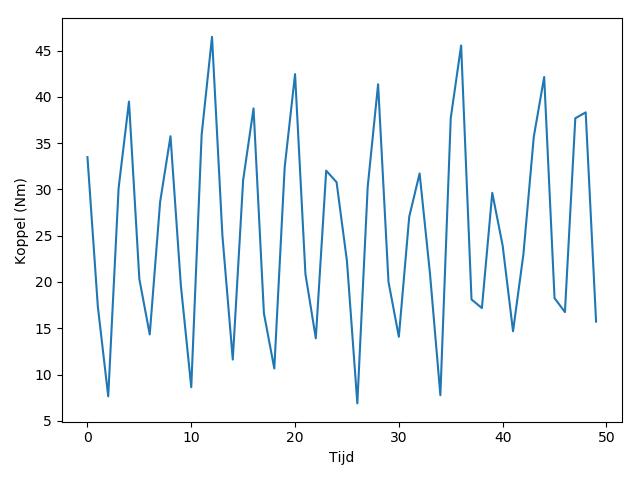
\includegraphics[width=\linewidth]{images/menselijkkoppel.png}
  \caption{Menselijk koppelverloop}
  \label{fig:menselijkkoppelverloop}
\end{subfigure}%
\begin{subfigure}{.5\textwidth}
  \centering
  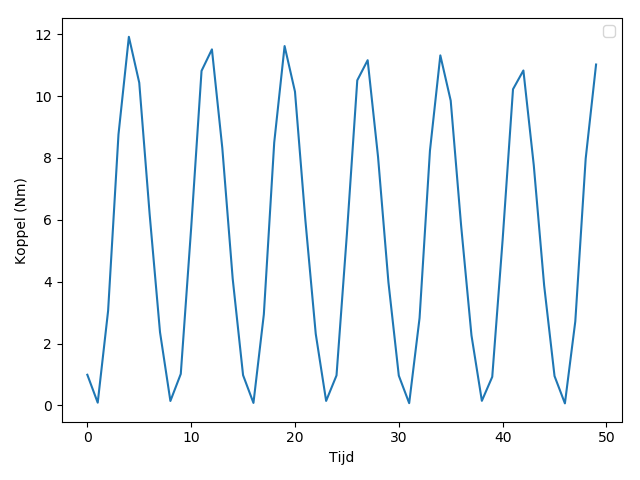
\includegraphics[width=\linewidth]{images/gesimuleerdekoppel.png}
  \caption{Gesimuleerd koppelverloop}
  \label{fig:gesimuleerdkoppelverloop}
\end{subfigure}
\begin{subfigure}{.5\textwidth}
  \centering
  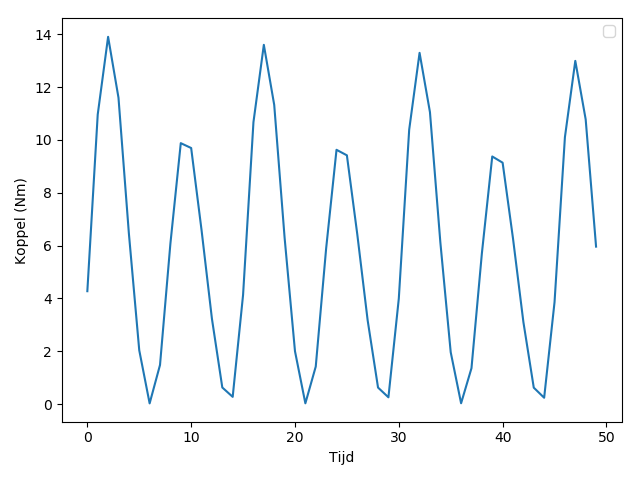
\includegraphics[width=\linewidth]{images/gesimuleerdekoppeldominantbeen.png}
  \caption{Gesimuleerd koppelverloop met dominant been}
  \label{fig:gesimuleerde koppel dominant been}
\end{subfigure}
\caption{Het koppelverloop van een mens (linksboven), de simulatie (rechtsboven) en een gesimuleerd dominant been (onderaan)}
\label{fig:koppelverloop mens-simulatie}
\end{figure}
\newpage
\begin{wrapfigure}{R}{0.5\textwidth}
  \centering
  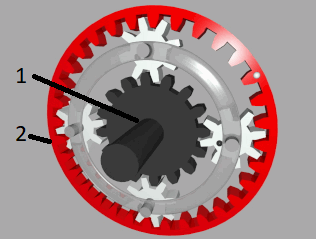
\includegraphics[width=\linewidth]{images/planeetwielmechanisme.png}
  \caption{Planeetwielmechanisme (bron: Wikipedia)}
  \label{fig:planeetwielmechanisme}
\end{wrapfigure}

\noindent $T_{cy}$ is het koppel op de trapas. Dit moet nog overgebracht worden op het achterwiel. Ellio maakt gebruik van een planeetwielmechanisme (figuur \ref{fig:planeetwielmechanisme}). Dit mechanisme laat toe om een grote overbrengingsverhouding te voorzien in een kleine ruimte. Het achterwielkoppel wordt beïnvloed door het aantal tanden op het zonnewiel (1; \gls{ns}) en het ringwiel (2; \gls{nr}) en de overbrengingsverhouding tussen de trapas en het ringwiel (\gls{k_cr,r}). Het koppel op het achterwiel (\gls{t_rw}) ziet er als volgt uit:
\begin{gather*}
T_{rw}=T_{cy}*k_{cr,r}*\frac{nr+ns}{nr}
\end{gather*}
\\\\
Bovenop het vermogen geproduceerd door de fietser, levert Ellio extra ondersteuning a.d.h.v. een motor (\gls{t_mg2}) gekoppeld aan het voorwiel. De fietser kan zelf een ondersteuningsniveau (\gls{s}) instellen tussen 0 en 5. Hoe hoger dit ondersteuningsniveau, hoe minder inspanning de fietser moet leveren. 
\begin{gather*}
T_{MG2}=min(35,S\thinspace .\thinspace T_{cy})
\end{gather*}

\subsection*{Het fietsersmodel}
Hoe kiest een fietser zijn cadans? Dit is voor elke fietser verschillend en er is nog nauwelijks onderzoek naar gebeurd. Wielrenners trainen om sneller te kunnen trappen omdat dit efficiënter is. Ze kunnen een gemiddeld vermogen leveren van 300 Watt. De doorsnee fietser levert gemiddeld ongeveer 75 Watt tijdens een normale fietstocht. Het fietsersmodel zal hierop worden afgesteld, aangezien wielrenners niet de voornaamste doelgroep zijn voor Ellio.
\\\\
Het fietsersmodel is een functie die op verschillende manieren uitgedrukt kan worden: op basis van de helling, gemiddeld koppel, of snelheid. Wat het correcte model is, wordt in deze thesis niet uitgewerkt. Het is vooral van belang dat de cadanscontroller het model zo snel en zo nauwkeurig mogelijk kan achterhalen, ongeacht wat het model precies is. Hier wordt de volgende aanname gemaakt: hoe hoger het koppel geleverd door de fietser, hoe hoger de gewenste cadans. Wanneer de fietser bijvoorbeeld een helling oprijdt, schakelt hij of zij een versnelling omlaag zodat de kracht die op de pedalen gezet moet worden aangenaam blijft. We stellen hier volgende eenvoudige modellen voor:
\begin{align*}
Gemiddeld \ koppel:\tab FCC &= \gls{f_k} . T_{dc}\\
Helling:\tab FCC &= \gls{f_h} . \alpha\\
Snelheid:\tab FCC &= \gls{f_v} . v_{bike}
\end{align*}
Er wordt verder aangenomen dat de fietser ook een zekere lineariteit verwacht bij lage snelheden (figuur \ref{fig:cadansverloop}). Dat wil zeggen dat een fietser het niet comfortabel vindt wanneer hij of zij snel moet trappen wanneer de fiets nog stilstaat of heel traag rijdt, ook al moet er op dat moment veel koppel geleverd worden om te kunnen vertrekken. Daarom wordt bij lage snelheden de FCC begrensd door een lineair oplopend maximum, te vergelijken met een mechanische fietsversnelling. Omdat de doorsnee fietser niet heel traag of heel snel trapt, wordt de FCC begrensd tussen de 40 en 120 rpm.
\begin{figure}
  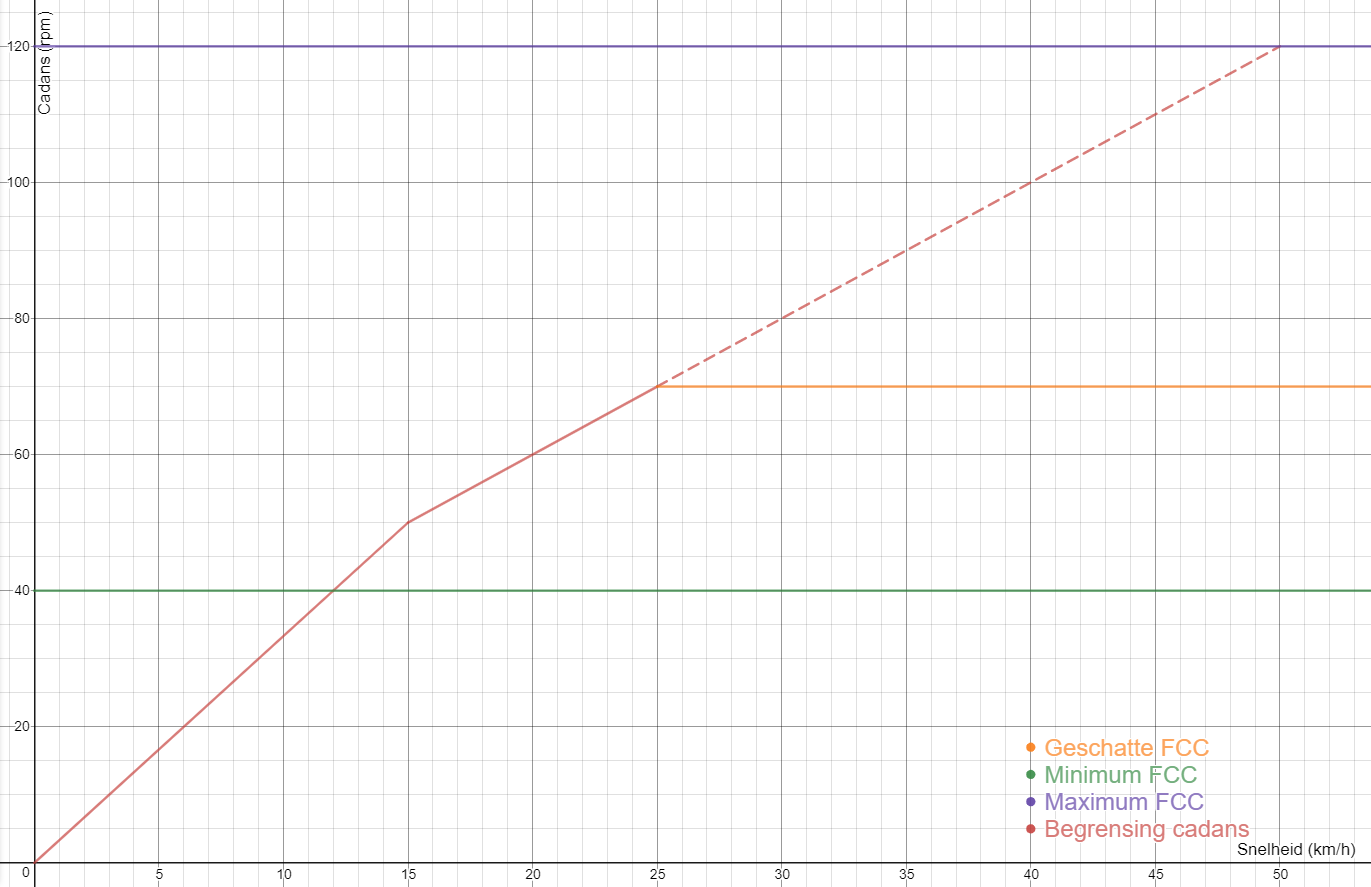
\includegraphics[width=\linewidth]{images/cadansverloop.png}
  \caption{Verwacht cadansverloop in functie van de snelheid.}
  \label{fig:cadansverloop}
\end{figure}
\newpage
\subsection*{Het lastmodel}
De simulatie is voorzien van een lastmodel. Zoals in realiteit, werken lasten in op de fiets. Zwaartekracht, wrijving met de weg en luchtweerstand zijn gemodelleerd als volgt:
\\
\begin{align*}
\gls{f_grav}&=\gls{m} \ . \ \gls{g} \ . \ sin \ \alpha \\
\gls{f_friction}&=m \ . \ g \ . \ \gls{c_r} \ . \ cos \ \alpha \\
\gls{f_aero}&=\frac{\gls{c_d} \ . \ \gls{rho_aero} \ . \ \gls{a_aero} \ . \ v_{bike}^2}{2}
\end{align*}
Samen vormen ze de totale belasting op de fiets.
\[\gls{f_load} = F_{grav}+F_{friction}+F_{aero}\]
Deze lasten zorgen ervoor dat de simulatie een realistische hoeveelheid vermogen nodig heeft om een bepaalde snelheid te halen. Er wordt hier geen rekening gehouden met de wind. Ten eerste zou dit extra complexiteit toevoegen aan de simulatie. Ten tweede vertrekken we van volgende hypothese:
\\\\
\tab De \textit{freely chosen cadence} hangt af van de hoeveelheid last, van welke bron dan \tab ook, die de gebruiker ondervindt.
\\\\
Het voorgestelde lastmodel omvat deze vereiste. Door de helling en referentiesnelheid te variëren ondergaat de fietser een veranderende last. Zoals in de realiteit zoeken mensen een bepaalde snelheid te halen. Wanneer de fietser een te hoge last ondervindt, bijvoorbeeld door een berg op te rijden, moet hij of zij meer vermogen genereren om zijn of haar gewenste snelheid te behouden. Hiervoor zijn 2 mogelijkheden: het verhogen van het koppel of de trapsnelheid. Mensen zijn meer geneigd om hun gewenste cadans te behouden, ongeacht het koppel (binnen bepaalde grenzen). De formule voor mechanisch vermogen gaat als volgt:
\[\gls{p}=T_{cy} \ . \omega_{cr} \]
Om het lastmodel correct te laten werken, moet er nog een helling gegenereerd worden. Om veel werk uit te sparen met het uitstippelen van parcours, wordt dit dynamisch gegenereerd met behulp van \textit{Perlin noise} (figuur \ref{fig:hellingverloop}). Perlin noise kan gebruikt worden om willekeurige getallen te genereren waarbij opeenvolgende getallen weinig van elkaar verschillen. Een perfecte kandidaat dus om terrein te simuleren. Om verschillende trajecten te creëren, kan de seed variabele aangepast worden. Een hellingsgraad wordt in de fietswereld vaak percentueel voorgesteld. Deze implementatie heeft echter radialen nodig. De helling zal beperkt worden tussen $\approx$ 0 en 10\% (0 en 0.1 radialen). Ter vergelijking, de Koppenberg heeft een gemiddeld stijgingspercentage van 11.6\%. Het minimum stijgingspercentage is zo gekozen dat de simulatie zo weinig mogelijk gaat freewheelen.
\begin{figure}[t]
  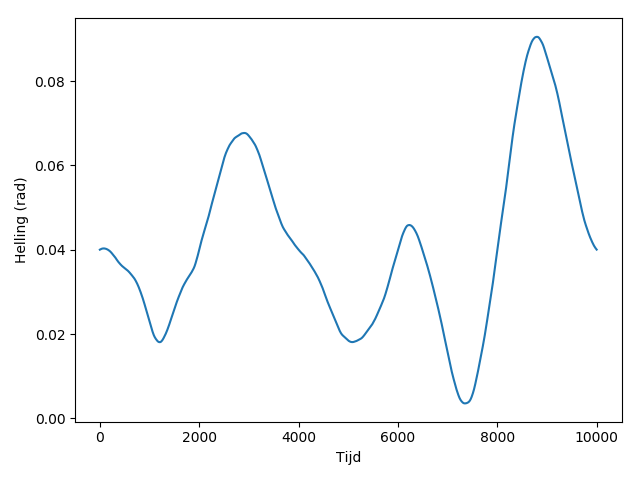
\includegraphics[width=\linewidth]{images/parcour_slope_example.png}
  \caption{Voorbeeld helling verloop}
  \label{fig:hellingverloop}
\end{figure}
\newpage
\subsection*{Snelheidsvergelijking}
\noindent De snelheid wordt geïntegreerd met een voorwaartse Euler methode. De acceleratie is een functie van de last, het totaalgewicht (m), het koppel geleverd door de fietser op het achterwiel ($T_{rw}$) en het koppel van een motor bevestigd op het voorwiel ($T_{MG2}$). 
\\\\
De bewegingsvergelijking van de fiets is, met inbegrip van het lastmodel en het fietsersmodel:
\[F \ = \  m \ . \ a \]
Deze vergelijking wordt elke tijdsstap geïntegreerd met behulp van een voorwaartse Euler methode:
\[F = m.(\frac{v_{bike}[h]-v_{bike}[h-1]}{\Delta t})\]
\[ \frac{F.\Delta t}{m}=v_{bike}[h]-v_{bike}[h-1]\]
\[v_{bike}[h]=v_{bike}[h-1]+\Delta t .\frac{1}{m}.F\]
\[v_{bike}[h] \ = \ v_{bike}[h-1] \ + \Delta t  \ . \frac{1}{m} \ . \ (\frac{T_{MG2} \ + \ T_{rw}}{r_w} \ - \ F_{load})\]
\newpage
De volledige simulatie ziet er als volgt uit:
\begin{algorithm}
\caption*{Fietssimulatie}
\For{$\text{h} = 1,\#tijdssprongen$}
{
$T_{dc,max} = \frac{-\omega_{cr}[h-1]}{2}+60$\\
$T_{dc} = min(T_{dc,max}, \ max(0,-K*(v_{bike}[h-1]-v_{ref})))$\\
$FCC = f(T_{dc})$\\
$\omega_{cr}=cadans(v_{bike}[h-1], \ T_{dc}, \ fcc)$\\
$\theta_{cr}=\theta_{cr}[h-1] + \Delta t \ . \ \omega_{cr}$ \\
$T_{cy} = T_{dc}(1+sin(2\theta_{cr}-\frac{\pi}{6}))$\\
$T_{rw}=T_{cy}*k_{cr,r}*\frac{nr+ns}{nr}$\\
$T_{MG2}=min(35, \ S \ . \ T_{cy})$\\
$F_{grav}=m \ . \ g \ . \ sin \ \alpha$\\
$F_{friction}=m \ . \ g. \ c_r \ . \ cos \ \alpha$\\
$F_{aero}=\frac{c_d \ . \ \rho_{aero} \ . \ A_{aero} \ . \ v_{bike}[h-1]^2}{2}$\\
$F_{load} = F_{grav}+F_{friction}+F_{aero}$\\
$v_{bike} \ = \ v_{bike}[h-1] \ + \Delta t  \ . \frac{1}{m} \ . \ (\frac{T_{MG2} \ + \ T_{rw}}{\gls{r_w}} \ - \ F_{load})$
}
\end{algorithm}

\section{Voorspellen van de cadans}
Een groot deel van de toestand van de fiets wordt berekend. Om een efficiënt algoritme te creëren moet enkel de relevante data bekeken worden. Zo worden de volgende attributen gebruikt: snelheid, koppel, hoek van de trapas en helling. 
\\

\begin{wrapfigure}{R}{0.40\textwidth}
  \centering
  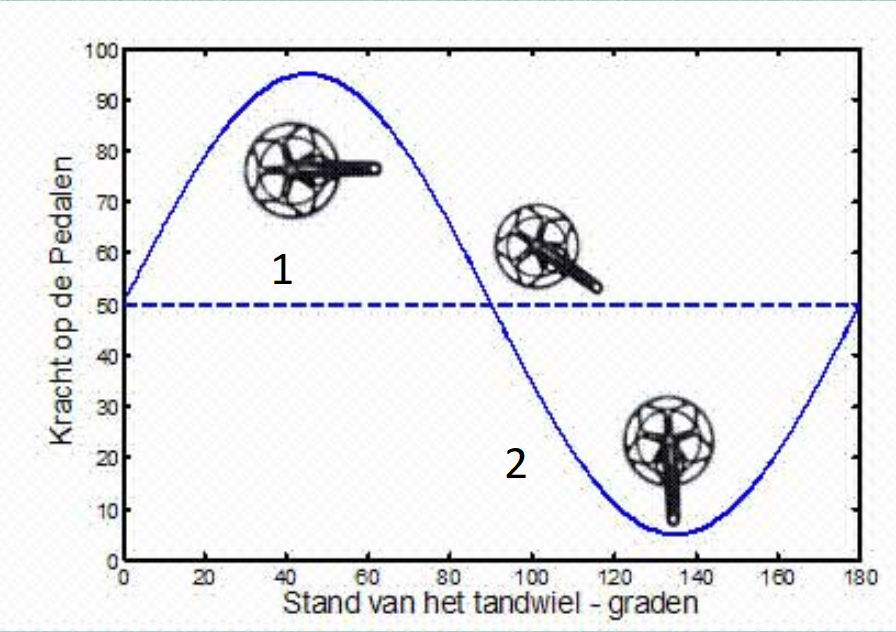
\includegraphics[width=\linewidth]{images/trapcyclus.png}
  \caption{Evolutie koppel in functie van hoek trapas (bron: fietsica.be)}
  \label{fig:Evolutie koppel in functie van hoek trapas}
\end{wrapfigure}
\noindent De helling is vanzelfsprekend. Dit is de voornaamste vorm van last en zal dus een impact hebben op de freely chosen cadence van de fietser. De hoek van de trapas en het koppel hebben individueel niet veel betekenis. Er kan bijvoorbeeld een koppel geleverd worden van 20Nm. Dit koppel kan op verschillende plaatsen geleverd worden in de trapcyclus. Als dit in de situatie 2 in figuur \ref{fig:Evolutie koppel in functie van hoek trapas} geleverd wordt, dan is dit waarschijnlijk het laagste koppel in de trapcyclus. Wordt dit geleverd gedurende de neergaande beweging (1), dan is dit het hoogste koppel. Deze verschillende situaties zullen een verschillende cadans nodig hebben. Tijdens de eerst situatie wordt er gemiddeld meer koppel geleverd, wat wijst op een grote last. Dus verwachten we hier een hoge cadans. De tweede situatie daarentegen zal gemiddeld een lagere last hebben. Daarom wordt in conjunctie met het koppel de hoek van de trapas gebruikt. Snelheid is ook een relevant attribuut. In situaties met verschillende snelheden en dezelfde last gaat de cadans verschillen.
\subsection*{Preprocessing}
Niet elk algoritme heeft nood aan genormaliseerde input. Voor algoritmes die een afstandsfunctie gebruiken is standaardisatie cruciaal. De doelvariabelen daarentegen moet niet genormaliseerd worden volgens Warren S. Sarle \cite{preprocessing faq}. In zijn FAQ schrijft hij dat het standaardiseren van de output voornamelijk voordelige effecten heeft op de initiële gewichten. Wanneer er meerdere doelvariabele zijn en als deze ver uit elkaar liggen, kan het wel nuttig zijn om ze te normaliseren. In dit geval is dat niet nodig aangezien enkel de cadans voorspeld zal worden.
\\\\
\noindent Ten eerste zal de data in sequentie gegoten worden. Een sequentie wordt gezien als een aantal vectoren ($x_t$) over verschillende tijdstippen. Een enkele data meting op zich is niet genoeg om een accurate voorspelling te maken, maar te veel data gebruiken is ook niet goed aangezien de voorspellingen tijdig moeten geleverd worden.
\\
\begin{gather*}
x_t = \begin{bmatrix} 
       \theta _{cr} \\ T_{cy,m} \\ v_{bike} \\ \alpha
     \end{bmatrix} \tab
sequentie = \begin{bmatrix} 
       x_t \\ x_{t-1} \\ ... \\ x_{t-n}
     \end{bmatrix} 
\end{gather*}
\\
\noindent Ten tweede zal de hoek van de trapas niet in zijn zuivere vorm gebruikt worden. De hoek van de trapas is een variabele tussen nul en $2 \pi$. Het probleem hier is dat het begin en het einde van een cyclus ver uit elkaar liggen. Voor de mens is het evident dat nul en twee pi hetzelfde zijn, maar voor de computer is dit een groot verschil. Daarom zal de sinus en de cosinus van de hoek genomen worden, zodat het begin en einde dicht bij elkaar liggen (figuur \ref{fig:preprocessing hoek trapas}). Zo leren we het algoritme bij dat de data zich cyclisch gedraagt.

\begin{figure}[h]
  \centering
  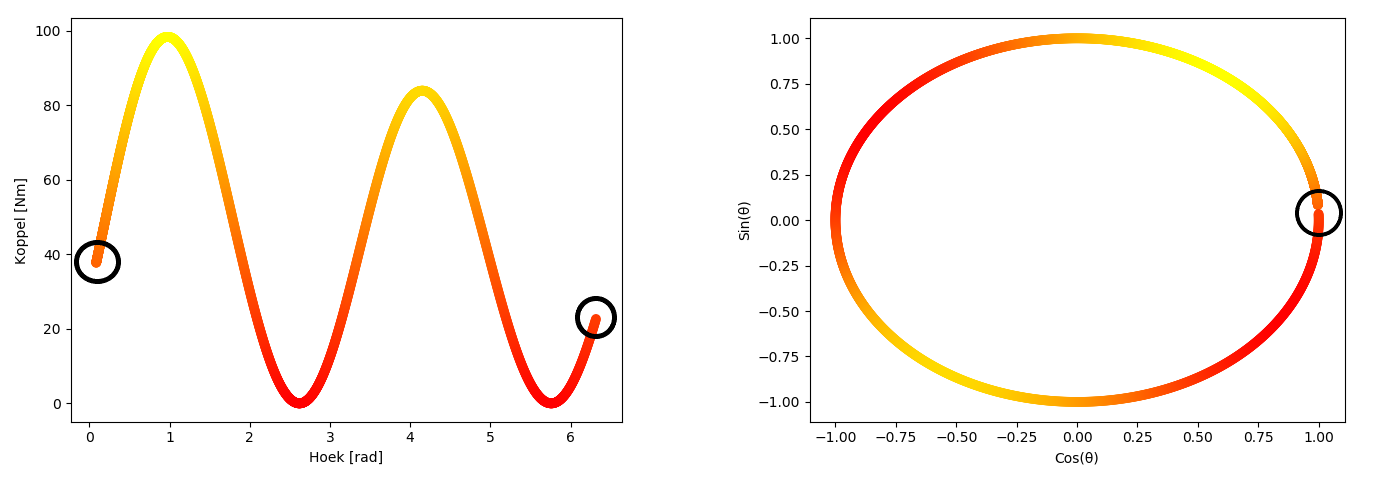
\includegraphics[width=\linewidth]{images/preprocessing-hoek.png}
  \caption{Figuur links toont dat het begin en einde van een trapcyclus ver uit elkaar liggen. Figuur rechts toont dat beide punten van de linkse figuur dicht bij elkaar liggen.}
  \label{fig:preprocessing hoek trapas}
\end{figure}

\noindent Ten slotte kan er ruis zitten op de metingen. Er zal altijd wel een klein foutje zitten op de data omdat de meetapparatuur niet perfect is. Het is mogelijk dat trillingen van de motor of het wegdek een impact kunnen hebben, voornamelijk op het geleverde koppel. Voor deze iteratie zal hier geen rekening mee gehouden worden. Ruis van het wegdek komt voor op een frequentie van ongeveer 20 Hz en hoger. Dit kan nog correct opgenomen worden als er op voorhand data wordt gesampled op hogere frequentie. Ruis van de motoren daarentegen komt voor op 13000 Hz, ver boven de sample frequentie en zal dus afgebeeld worden op lagere frequenties. Het huidige systeem zal geen rekening houden met beide soorten ruis. Om de gevoeligheid voor ruis te minimaliseren kan het ingangssignaal eenvoudig gefilterd worden met een laagdoorlaatfilter van bijvoorbeeld 10 Hz. Figuur \ref{fig:fft fietser} toont een \textit{fast fourier transformatie} van het menselijk koppelverloop.

\begin{figure}[h]
  \centering
  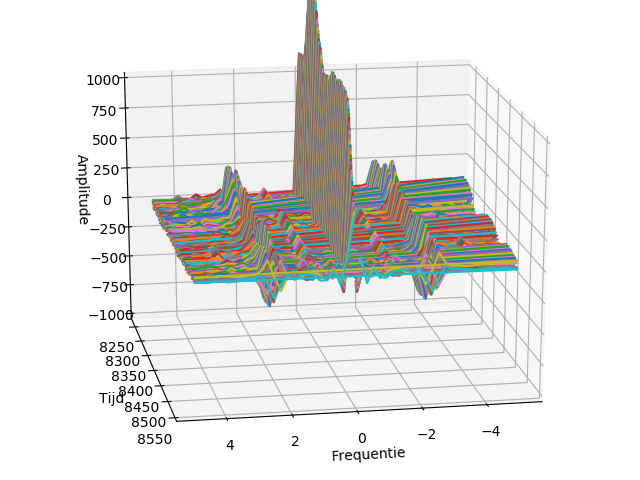
\includegraphics[width=\linewidth]{images/fft_fietser.png}
  \caption{Een Fast Fourier Transformatie van het menselijk koppelverloop.}
  \label{fig:fft fietser}
\end{figure}

\subsection*{Algoritmes}
\subsubsection*{Passive Aggressive algorithm}
Het \gls{pa} algoritme, beschreven in de paper van Crammer et al. \cite{pa algorithm}, is een on-line algoritme gelijkaardig aan een perceptron. Net zoals de perceptron, doet PA de matrixvermenigvuldiging $y_t=w_t \cdot x_t$ om de voorspelling te berekenen. Het grootste verschil tussen beide is hoe de gewichten geüpdatet worden. Het PA algoritme is bruikbaar voor classificatie, regressie, uniclass voorspellingen en multiclass problemen.
\\\\
\noindent Het PA algoritme, zoals de naam weggeeft, kan zich zowel passief als agressief gedragen. Het trainen van PA bestaat uit twee stappen. In de eerste stap wordt er een voorspelling $y_{t,p}$ gemaakt a.d.h.v. de input vector $x_t$ en gewichtenmatrix $w$. Hierna wordt het echte label $y_t$ bekendgemaakt. Als de fout kleiner is dan een voorgedefinieerde waarde $\epsilon$, dan zullen de gewichten niet geüpdatet worden. Als de error toch groter is dan deze marge, dan zullen de gewichten $w$ aangepast worden zodat de fout voor de huidige instantie nul wordt. PA past de gewichten aan zodat het verschil tussen het vorige gewicht en het nieuwe gewicht minimaal is. 
\[
    loss_{\epsilon} (w_t;(x_t,y_t))=\left\{
                \begin{array}{ll}
                  0 \tab \tab \tab \ \ |w \cdot x - y| \leq \epsilon \\
                  |w \cdot x - y| - \epsilon \tab anderzijds
                \end{array}
              \right.\\
\]
\[
    w_{t+1}= \argmin_{w \in \mathbb{R}^n}
     \frac{1}{2}||w-w_t||^2 \tab zodat \ loss_{\epsilon} (w_{t+1};(x_t,y_t)) = 0
\]
Door de agressiviteit van het standaard PA algoritme kunnen er problemen ontstaan wanneer er veel ruis zit op de data. Daarom heeft Crammer et al. twee extra versies, PA-I en PA-II, gemaakt die dit probleem oplossen. Beide versies voegen een slack variabele $\xi$ toe. Deze variabele zorgt ervoor dat bij het aanpassen van de gewichten, de fout kleiner of gelijk moet zijn aan $\xi$ in plaats van nul. Beide versies hebben ook een agressiviteits parameter C die deze $\xi$ beïnvloedt. Dit is een vorm van regularisatie om overfitting te voorkomen.

\[
   PA-I \tab w_{t+1}= \argmin_{w \in \mathbb{R}^n}
     \frac{1}{2}||w-w_t||^2 + C\xi \tab zodat \ loss_{\epsilon} (w_{t+1};(x_t,y_t)) \leq \xi
\]
\[
   PA-II \tab w_{t+1}= \argmin_{w \in \mathbb{R}^n}
     \frac{1}{2}||w-w_t||^2 + C\xi^2 \tab zodat \ loss_{\epsilon} (w_{t+1};(x_t,y_t)) \leq \xi
\]

De nieuwe gewichtenmatrix $w_{t+1}$ wordt als volgt berekend:
\[
w_{t+1}=w_t+ \tau_t y_t x_t
\]
\begin{align*}
\tau_t &= \frac{loss_t}{||x_t||^2} \tab \tab (PA)\\
\tau_t &= min \{ C, \frac{loss_t}{||x_t||^2} \} \ \ (PA-I)\\
\tau_t &= \frac{loss_t}{||x_t||^2+\frac{1}{2C}} \tab (PA-II) 
\end{align*}


\subsubsection*{Decision Tree en Random Forest}
Een \gls{dt} is een regel-gebaseerd model (\textit{rule-based model}). Dit algoritme is snel (\textit{greedy}), maar kan niet goed om met ruis. Dit model is gekend om makkelijk te overfitten. Daarom wordt het \gls{rf} algoritme simultaan bekeken.
\\\\
Een DT is een binaire boom. In elke knoop wordt een binair keuzepunt gemaakt op basis van een attribuut. Dit keuzepunt is gekozen zodat de data optimaal gesplitst is over beide takken. \texttt{Sci-kit learn} biedt de mogelijkheid aan om de maximum diepte van de boom te beperken. Wanneer deze parameter niet ingesteld is, zal de DT blijven groeien totdat alle blad nodes ``puur" \ zijn. Een correcte diepte kiezen is een enorm moeilijke taak.
\\\\ 
RF is een ensemble. Dit wilt zeggen dat meerdere algoritmes, in dit geval meerdere DT’s, gebruikt worden om een betere voorspelling te maken. L. Breiman \cite{randomforest paper} beweert in zijn paper dat alle RF’s convergeren zodat overfitting geen probleem is. In tegenstelling tot DT’s, kiest een RF geen optimaal attribuut wanneer een node gesplitst wordt. De variabele worden at random gekozen, waardoor geen enkele boom dezelfde is. De verschillende bomen trainen niet met exact dezelfde trainingsdata. Ze passen Bootstrap Aggregating toe, of bagging. Dit houdt in dat uit de originele trainingsset data wordt gesampled at random. Een instantie kan meerdere keren gesampled worden. Deze techniek reduceert de variantie.
\subsection*{Post-processing}
De cadans variëert lichtjes doorheen een trapcyclus, zowel in het echt als in de simulatie. De voorspellingen zullen dezelfde trend vertonen. Bovendien kan een beetje ruis of het gedrag van de fietser voor afwijkingen zorgen, bijvoorbeeld een grote sprong tussen twee voorspellingen. Dit kan ergerend zijn voor de fietser.
\\\\
Dit probleem kan op verschillende manieren opgelost worden. Gebruikmakend van de huidige en vorige voorspellingen (\gls{fcc_pred}) of de vorige schatting ($FCC_{est}$). De vorige instelling is de cadans die is doorgegeven aan de fiets controller.
\begin{align*}
\gls{ma} \tab  FCC_{est,t} &= \frac{\sum_{i=0}^{n} FCC_{pred,t-i} }{n}\\
\gls{es} \tab FCC_{est,t} &= \gls{sf} . FCC_{pred,t} + (1-sf) . FCC_{est,t-1}
\end{align*}
MA lost beide problemen goed op. Meer voorspellingen leidt tot stabielere schattingen, maar dit introduceert een vertraging (\textit{lag}) op de cadans. Namelijk wanneer de omstandigheden veranderen, zal de ingestelde cadans slechts na enkele iteraties optimaal zijn, in plaats van onmiddellijk. ES vermindert de amplitude van de oscillaties slechts in mindere mate. Figuur \ref{fig:effecten postprocessing} toont wat de impact is van ES en MA op ruizige voorspellingen (20\% kans op ruis tussen -10 en +10).
\begin{figure}[!t]
\centering
\begin{subfigure}{.5\textwidth}
  \centering
  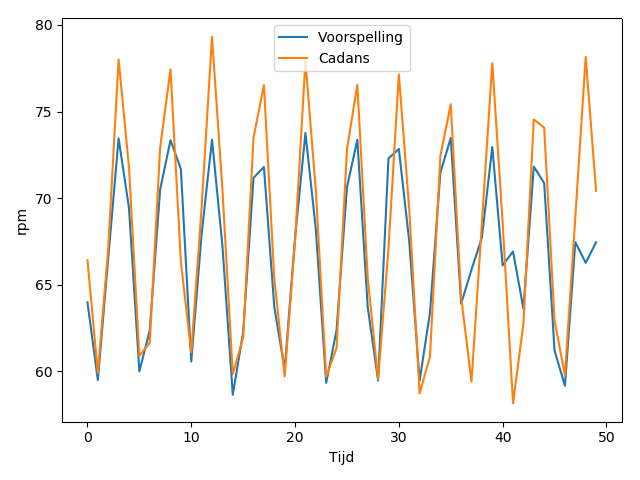
\includegraphics[width=\linewidth]{images/actual-prediction+noice,nopp.png}
  \caption{Geen post-processing}
  \label{fig:geen postprocessing}
\end{subfigure}%
\begin{subfigure}{.5\textwidth}
  \centering
  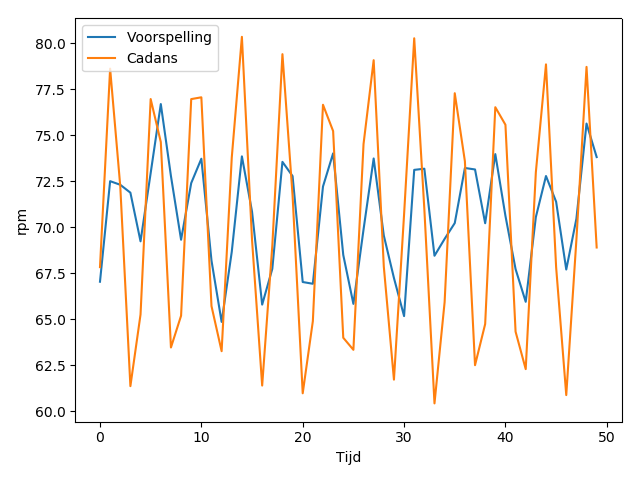
\includegraphics[width=\linewidth]{images/actual-prediction+noice,es.png}
  \caption{Exponential Smoothing}
  \label{fig:exponential smoothing postprocessing}
\end{subfigure}
\begin{subfigure}{.5\textwidth}
  \centering
  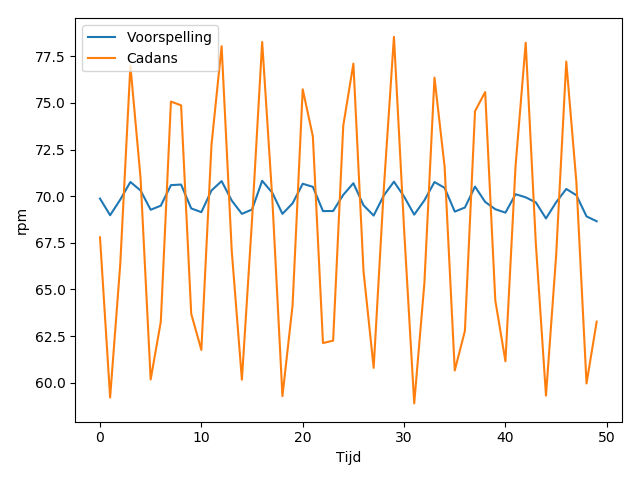
\includegraphics[width=\linewidth]{images/actual-prediction+noice,ma.png}
  \caption{Moving Average}
  \label{fig:moving average postprocessing}
\end{subfigure}
\caption{De effecten van verschillende post-processing technieken.}
\label{fig:effecten postprocessing}
\end{figure}
\newpage
\section{Stochastisch bijleren}
Het volgende hoofdstuk van deze thesis bespreekt de experimentele resultaten. In deze testen leren de algoritmes op een deterministische manier bij. Een mens daarentegen is onvoorspelbaar. Soms is de fietser snel geërgerd en drukt hij sneller op de knop om zijn cadans aan te passen. Soms vindt hij een incorrecte cadans niet erg genoeg om daarvoor op de knop te duwen. Dit zou gesimuleerd moeten worden om te achterhalen of de modellen met dit non-determinisme omkunnen. 
\\\\
Net zoals volgens de deterministische update-strategie, zal het fietsersmodel als de waarheid genomen worden. Hoe groter het absoluut verschil is tussen de cadans en het fietsersmodel (\gls{delta_c}), hoe hoger de kans dat de fietser effectief op de knop zal duwen waardoor het model kan bijleren. De probabiliteit van het bijleren, hier $P(u_c|\Delta_c)$, zal lineair evolueren. Wanneer het verschil zich bevindt tussen nul en vijf, schaalt de kans lineair mee van 0\% naar 20\% kans. Wanneer deze grens overschreden wordt, groeit de kans sneller mee tot 100\% kans wanneer het verschil groter of gelijk is aan tien (figuur \ref{fig:kansverdeling cadansupdate}). Deze strategie is bedoeld voor een simulatie gesampled aan één Hertz. Als de frequentie verhoogt naar bijvoorbeeld 10000 Hz, evolueert dit stochastische beslissingsmodel naar een deterministische, aangezien er enorm vaak een kans is op de updaten. Daarom moet $P(u_c|\Delta_c)$ nog vermenigvuldigd worden met de grootte van de tijdstap (x0,1 voor 10 Hz). Of het vermenigvuldigen van de frequentie met de probabiliteit van updaten correct is, is evident aan te tonen met behulp van de verwachtingswaarde over een binomiale verdeling (met $\Delta_c=5$) \cite{binomial wiki}:
\begin{align*}
E(u_c|\Delta_c)_{1hz} \ &=p(u_c=1|\Delta_c)_{1hz} \\
E(u_c|\Delta_c)_{1hz} \ &=0.2 \\
E(u_c|\Delta_c)_{10hz}&=10*p(u_c=1|\Delta_c)_{10hz} \\
E(u_c|\Delta_c)_{10hz}&=0.2
\end{align*}

\begin{figure}[h]
  \centering
  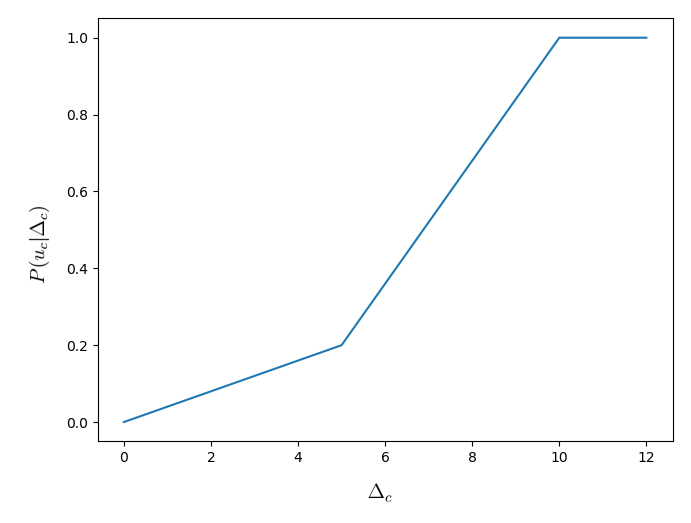
\includegraphics[width=\linewidth]{images/stochastische_kans_cadansupdate.png}
  \caption{Het verloop van de kansverdeling in functie van $\Delta_c$}
  \label{fig:kansverdeling cadansupdate}
\end{figure}

\noindent Hoe lang het gemiddeld duurt om bij te leren kan ook achterhaald worden met behulp van de verwachtingswaarde, deze keer als een geometrische distributie \cite{geometric wiki}. Het verschil tussen een binomiale distributie en een geometrische distributie is als volgt: een binomiale distributie is een kansverdeling over het aantal successen met kans $p$ na $k$ onafhankelijke testen. Een geometrische distributie vertelt iets over wat de kans is dat na $k$ pogingen, zodat de laatste poging een succes is met de kans op succes $p$ constant. Bijvoorbeeld: wat is de kans dat de simulatie na tien iteraties aan 10 Hz een update zal doorvoeren als $\Delta_c=5$?

\[p(u_c=10|\Delta_c=5)=(1-p)^9*p=0.98^9*0.02=0.01667\]
\\\\
\noindent Het gemiddeld aantal iteraties dat de simulatie nodig zou hebben om een update door te voeren, komt neer op het uitwerken van volgende oneindige reeks:
\begin{align*}
E(X)&=\sum_{k=1}^{\infty} (1-p)^kpk \\
E(X)&=p+2(1-p)p+3(1-p)^2 p...
\end{align*}
Wat neerkomt op:
\[E(X)=\frac{1}{p}\]
Voor een $\Delta_c$ van vijf zal het dus gemiddeld 5 iteraties (aan 1 Hz) en 50 iteraties (aan 10 Hz) duren vooraleer er geüpdatet wordt.
\\\\
Ten slotte wordt deze strategie beperkt, zodat het onmogelijk is om direct twee keer na elkaar op de knop te duwen. Dit is geïmplementeerd via een simpele controle van het verschil in tijd tussen de huidige iteratie en de iteratie van de vorige update.

\subsection{Verwachtingen}
We verwachten dat alle modellen dit stochastisch probleem aankunnen, omdat het verschil tussen fietsersmodel en cadans uiteindelijk groot genoeg zal worden zodanig dat het zeer onwaarschijnlijk is dat er niet op de knop geduwd wordt. Wat we hiermee willen bedoelen is dat het statistisch onwaarschijnlijk is dat er niet wordt bijgeleerd wanneer het verschil vergroot.
\section{Conceptuele drift}
Conceptuele drift is de verandering van het concept, in dit geval het fietsersmodel, na verloop van tijd. Deze verandering kan op verschillende manieren gebeuren: abrupt, geleidelijk en terugkerend. De FCC van een mens is een vorm van geleidelijke drift. Volgens Hansen et al. \cite{factors effecting cadence} heeft de leeftijd invloed op de FCC, zijnde oudere mensen trappen in het algemeen trager. De snelheid waaraan de FCC daalt, is enorm klein. Het gaat hier om drie rpm per decennium. Eens de fiets is ingesteld, zou er dus technisch gezien nooit meer moeten bijgeleerd worden, tenzij de fiets verandert van eigenaar. Dit is een vorm van abrupte drift, aangezien twee individuën hoogstwaarschijnlijk niet dezelfde FCC hebben. Deze sectie onderzoekt welke technieken er zijn om met deze abrupte drift om te gaan. Het doel van deze sectie is om een techniek te achterhalen die ervoor zorgt dat het gedrag van een tweede gebruiker zo snel mogelijk bijgeleerd is zonder de ervaring van de eerste gebruiker, die de fiets heeft gekocht, te verslechteren (het laatste is belangrijker voor IntuEdrive).
\\\\
Standaard hebben algoritmes van machinaal leren geen manier om met een drift om te gaan. Als het concept verandert, zal het nieuwe concept geleidelijk aan een groter aandeel krijgen in de trainingsset, met als gevolg dat het algoritme van machinaal leren uiteindelijk het nieuwe concept leert. Hierdoor kan het lang duren vooraleer het nieuwe concept goed voorspeld kan worden. Een techniek om met conceptuele drift om te gaan, is het vergeten van oude data (het oude concept). In dit deel zullen drie technieken besproken worden die Loeffel \cite{adaptive ml} in zijn doctoraat aanhaalt. Statisch schuivend venster (\textit{fixed sliding window}) en een sampling techniek zijn zelf geïmplementeerd zoals beschreven door Loeffel \cite{adaptive ml} en Aggarwal \cite{biased reservoir sampling} respectievelijk.
\subsection{Statisch schuivend venster (\textit{static sliding window})}
Een statisch schuivend venster is de simpelste techniek om een vergeetmechanisme toe te voegen aan een algoritme van machinaal leren voor abrupte drifts. Een statisch schuivend venster is een set van de $n$ meest recente elementen in een data stroom. Wanneer er data in het schuivend venster zit, nemen we aan dat dit het meest recente concept vertegenwoordigt. Mocht het concept plots veranderen, en het schuivend venster zit vol, dan zal de oude data plaats maken voor de nieuwe data waardoor het oude concept na verloop van tijd vergeten wordt.
\setcounter{table}{0}
\begin{table}[h]
\begin{tabular}{|c|l|}
\hline
\multicolumn{2}{|c|}{Statisch schuivend venster} \\ \hline
Voordelen & \multicolumn{1}{c|}{Nadelen} \\ \hline
\multicolumn{1}{|l|}{\begin{tabular}[c]{@{}l@{}}+ Simpel\\ + Start meteen met vergeten op het moment \\ \phantom{+} van de conceptuele drift\\ + Groot venster maakt het model robuust \\ \phantom{+} tegen ruis en zorgt voor een accuraat en \\ \phantom{+} stabiel model\\ \phantom{test} \end{tabular}} & \begin{tabular}[c]{@{}l@{}} - Een correcte grootte voor het venster \\  \phantom{-} is moeilijk te vinden\\ - Een te klein venster kan mogelijk het \\ \phantom{-} concept niet goed omvatten\\ - Een te groot venster vergeet trager\\ - Ruis kan goede, relevante data uit \\ \phantom{-} het venster verwijderen\end{tabular} \\ \hline
\end{tabular}
\caption{Voor- en nadelen van statisch schuivend venster}
\label{tab:voor- en nadelen van fixed sliding window}
\end{table}
\subsection{Variabel schuivend venster (\textit{variable sliding window})}
Een variabel schuivend venster is gelijkaardig aan een statisch schuivend venster. Het enige verschil is dat de grootte van het venster kan variëren. Dit mechanisme introduceert een veranderingsdetector (\textit{change detector}), een algoritme dat moet uitmaken of het concept verandert of niet. Als de change detector geen verandering opmerkt (zelfde concept), zal het venster vergroten. Daardoor stijgt het aantal elementen van het huidige concept. Dit brengt het voordeel met zich mee dat het model meer trainingsdata heeft en daardoor accurater en robuuster is. Eens de change detector opmerkt dat het concept verandert, dan zal de lengte van het venster verkleinen waardoor het een grote hoeveelheid data vergeet. Dit zorgt ervoor dat het model snel het nieuwe concept kan bijleren. Dit is wel een riskante strategie. De change detector kan geactiveerd worden met ruizige data (\textit{“catastrophic forgetting”}). Dit mechanisme kan bovendien ook niet goed om met een zeer trage drift, al is dit hier niet van belang. Omwille van het risico zal deze strategie niet uitgewerkt worden.

\begin{table}[!ht]
\begin{tabular}{|c|l|}
\hline
\multicolumn{2}{|c|}{Variabele schuivend venster} \\ \hline
Voordelen & \multicolumn{1}{c|}{Nadelen} \\ \hline
\multicolumn{1}{|l|}{\begin{tabular}[c]{@{}l@{}}+ Groot venster maakt het model robuust \\ \phantom{+} tegen ruis en zorgt voor een accuraat en \\ \phantom{+} stabiel model\\ + Kan venster verkleinen zodat het \\ \phantom{+} nieuwe concept snel bijgeleerd wordt\\ + Change detector kan ervoor zorgen dat\\ \phantom{+} een model hergebruikt kan worden (als\\\phantom{+} hetzelfde concept terugkeert) \\ \phantom{test}\end{tabular}} & \begin{tabular}[c]{@{}l@{}}- Een change detector implementeren is \\ \phantom{-} complex\\ - Riskante strategie\\ - Onnauwkeurige change detector zorgt voor\\ \phantom{-} problemen\\ - Change detector werkt met een drempel-\\\phantom{-} waarde voor detectie. Te klein en er kan een \\ \phantom{-} vals alarm optreden. Te groot en het zal te \\ \phantom{-} traag reageren\end{tabular} \\ \hline
\end{tabular}
\caption{Voor- en nadelen van variabel schuivend venster}
\label{tab:voor- en nadelen van variabele sliding window}
\end{table}
\newpage
\subsection{Sampling}
Ten slotte kan er gesampled worden om een relevante trainingset te genereren. Om een bias te krijgen voor recentere data zou een kansverdeling gebruikt kunnen worden met een bias naar recentere data. Dit is echter een naïeve implementatie die veel geheugen inneemt, aangezien alle trainingsdata moet bijgehouden worden. In de paper van Aggarwal C. \cite{biased reservoir sampling} worden twee technieken voorgesteld die data van een stream samplen met een bias voor recente data. Beide technieken zijn gebaseerd op reservoir sampling.

\subsubsection{Reservoir sampling}
Reservoir sampling is een sampling strategie waar er gesampled wordt uit een stream $S$. Voor elk element $x \in S$, willen we een gelijke kans hebben dat dit element $x$ gesampled wordt. Stel dat er $k$ elementen gesampled moeten worden, dan zal de probabiliteit voor elk element gelijk zijn aan $k/|S|$. Het probleem hier is dat we niet weten hoe groot $S$ precies is. Bovendien is het mogelijk dat niet alle elementen van $S$ in geheugen passen. Vitter J. \cite{reservoir sampling} lost dit op met een eenvoudig algoritme R.

\begin{algorithm}
\caption*{R}
$R = \bot \text{ met capaciteit }k$\\
$t=0$\\
\While{data stream S heeft nog elementen}
{
$t++$\\
\uIf{$t<k$}
{$A[t]=S[t]$}
\Else{
$i = random(0,t)$\\
\If{$i<=k$}
{$A[i]=S[t]$}
}
}
\end{algorithm}

\newpage
\begin{figure}[htp!]
  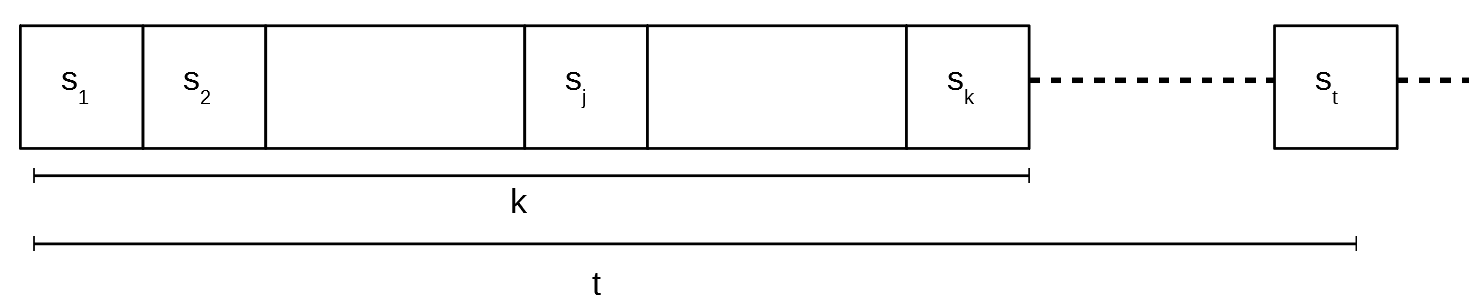
\includegraphics[width=\linewidth]{images/reservoir_sampling_voorbeeld.png}
\caption{Reservoir sampling voorstelling}
  \label{fig:reservoir sampling voorbeeld}
\end{figure}

\noindent Hypothese: $P(s_t \in R) = \frac{k}{n}$ \\
Bewijs:
\begin{align*}
P(s_t \in R) &= \frac{k}{t} * (1-\frac{1}{t+1})* (1-\frac{1}{t+2})*...*(1-\frac{1}{n}) 
\\
P(s_t \in R) &= \frac{k}{t} * (\frac{t+1-1}{t+1})* (\frac{t+2-1}{t+2})*...*(\frac{n-1}{n})
\\
P(s_t \in R) &= \frac{k}{\text{\st{t}}} * (\frac{\text{\st{t}}}{\text{\st{t+1}}})* (\frac{\text{\st{t+1}}}{\text{\st{t+2}}})*...*(\frac{\text{\st{n-1}}}{n})\\
P(s_t \in R) &= \frac{k}{n}
\end{align*}

\subsubsection{Bevoordeelde reservoir sampling (\textit{biased reservoir sampling})}
Aggarwal C. \cite{biased reservoir sampling} introduceert een bias in reservoir sampling.

\begin{algorithm}
\caption*{Bevoordeelde reservoir sampling}
$R = \bot \text{ met capaciteit }k$\\
$t=0$\\
\While{data stream S heeft nog elementen}
{
$t++$\\
$f=\text{de volheid van R, zijnde een getal tussen }[0,1]$\\
$i = random(0,1)$\\
Voeg element S[t] toe aan R\\
\If{$i<=f$}
{Verwijder een willekeurig element uit R}
}
\end{algorithm}
\noindent In zijn paper geeft Aggarwal aan dat de kans dat een element in $R$ zit exponentieel daalt in functie van $t$. Dit wil zeggen dat oudere elementen een exponentieel kleinere kans hebben om in $R$ te zitten dan recente elementen. De probabiliteit gaat als volgt, met $r$ het r-de punt in $R$, $t$ het t-de punt in S en \gls{lambda} een bias ratio die applicatie specifiek is:
\[f(r,t)=e^{-\lambda(t-r)}\]
De bias ratio $\lambda$ wordt bepaald aan de hand van de grootte van het reservoir (k):
\[\lambda=\frac{1}{k}\]

\begin{table}[!ht]
\begin{tabular}{|c|l|}
\hline
\multicolumn{2}{|c|}{Bevoordeelde reservoir sampling} \\ \hline
Voordelen & \multicolumn{1}{c|}{Nadelen} \\ \hline
\multicolumn{1}{|l|}{\begin{tabular}[c]{@{}l@{}}+ Geheugen efficiënt\\ + Kan een diverse set van data beter leren\\ \phantom{+} (data die verder uit elkaar ligt, heeft \\ \phantom{+} meer betekenis dan twee observaties vlak\\ \phantom{+} na elkaar)\\ + Het achterliggende model kan efficiënter \\ \phantom{+} worden omdat er minder data opgeslagen\\ \phantom{+} wordt\end{tabular}} & \begin{tabular}[c]{@{}l@{}}- Als het concept vaak verandert, heb je het\\ \phantom{-} ``van alles iets" \ probleem\\ - Het kan zijn dat het oude concept nog voor\\ \phantom{-} een lange tijd in het reservoir zit\\ \phantom{test} \\ \phantom{test}\\ \phantom{test}\\ \phantom{test}\end{tabular} \\ \hline
\end{tabular}
\caption{Voor- en nadelen van bevoordeelde reservoir sampling}
\label{tab:voor- en nadelen van biased reservoir sampling}
\end{table}
\newpage
\subsection{Verwachtingen}
Er wordt verwacht dat kleinere datastructuren (klein venster of reservoir), die net groot genoeg zijn om één concept te omvatten, slechter zullen presteren dan grotere datastructuren. Het is namelijk mogelijk dat relevante informatie te snel uit het geheugen zal verdwijnen. De eerste observaties van het nieuwe concept zouden al uit het geheugen verwijderd kunnen zijn voordat het concept geleerd is.
\\\\
In het algemeen verwachten we dat sampling beter zal presteren dan een statisch schuivend venster, aangezien observaties langer in het geheugen blijven. Ik denk dat dit het “vergeten” niet gaat tegenwerken, omdat het oude observaties geleidelijk aan verwijderd. Als een statisch schuivend venster en sampling dezelfde grootte hebben, dan zal data van update $u_t$ na $k$ updates helemaal uit het geheugen verwijderd zijn. Dit is niet het geval bij sampling. Data kan langer dan $k$ updates in het geheugen blijven, maar steeds in een kleinere hoeveelheid.
